\documentclass{beamer}

\usepackage{graphicx}
\usepackage{textpos}
\usepackage{listings}
\usepackage{lstautogobble}

\usetheme{Madrid}
\useoutertheme{miniframes} % Alternatively: miniframes, infolines, split

% Setup the university's color pallette
\definecolor{UIUCorange}{RGB}{19, 41, 75} % UBC Blue (primary)
\definecolor{UIUCblue}{RGB}{232, 74, 39} % UBC Grey (secondary)

\definecolor{codegreen}{rgb}{0,0.6,0}
\definecolor{codegray}{rgb}{0.5,0.5,0.5}
\definecolor{codepurple}{rgb}{0.58,0,0.82}
\definecolor{backcolour}{rgb}{0.95,0.95,0.92}

\lstdefinestyle{python}{
  backgroundcolor=\color{backcolour},   
  commentstyle=\color{codegreen},
  keywordstyle=\color{magenta},
  numberstyle=\tiny\color{codegray},
  stringstyle=\color{codepurple},
  basicstyle=\ttfamily\footnotesize,
  breakatwhitespace=false,         
  belowskip=-0.5em,
  breaklines=true,                 
  captionpos=b,                    
  keepspaces=true,                 
  numbers=left,                    
  numbersep=5pt,                  
  showspaces=false,                
  showstringspaces=false,
  showtabs=false,                  
  tabsize=2
}

\lstset{style=python}

\AtBeginSection[]{
    \begin{frame}
        \vfill
        \centering
        \begin{beamercolorbox}[sep=8pt,center,shadow=true,rounded=true]{title}
            \usebeamerfont{title}\insertsectionhead\par%
        \end{beamercolorbox}
        \vfill
    \end{frame}
}
% Setup the university's color pallette
\definecolor{UIUCorange}{RGB}{19, 41, 75} % UBC Blue (primary)
\definecolor{UIUCblue}{RGB}{232, 74, 39} % UBC Grey (secondary)


\setbeamercolor{palette primary}{bg=UIUCorange,fg=white}
\setbeamercolor{palette secondary}{bg=UIUCblue,fg=white}
\setbeamercolor{palette tertiary}{bg=UIUCblue,fg=white}
\setbeamercolor{palette quaternary}{bg=UIUCblue,fg=white}
\setbeamercolor{structure}{fg=UIUCorange} % itemize, enumerate, etc
\setbeamercolor{section in toc}{fg=UIUCblue} % TOC sections

\setbeamercolor{subsection in head/foot}{bg=UIUCorange,fg=UIUCblue}
\setbeamercolor{subsection in head/foot}{bg=UIUCorange,fg=UIUCblue}

\usepackage[utf8]{inputenc}
\usepackage{graphicx}

%Information to be included in the title page:
\title{\textbf{Strings and Files}}
\author{\textbf{David H Smith IV}}
\institute[\textbf{UIUC}]{\textbf{University of Illinois Urbana-Champaign}}
\date{\textbf{Wed, July 13 2021}}

\setbeamertemplate{title page}[default][colsep=-4bp,rounded=true]
\addtobeamertemplate{title page}{\vspace{3\baselineskip}}{}
\addtobeamertemplate{title page}{
  \begin{textblock*}{\paperwidth}(-1.0em, -1.2em)
    
\includegraphics[width=\paperwidth, height=\paperheight]{imgs/uiuc.png}
  \end{textblock*} 
}{}

\begin{document}

\frame{\titlepage}

\section{Reminders}

%
% Slide 1
%
\begin{frame}
  \frametitle{Reminders}
  The following are due Friday
  \begin{itemize}
    \item Homework 9p1
    \item Participation 9p2
    \item Post-reading 9p2
  \end{itemize}
\end{frame}

\section{Files}
%
% Slide 2
%
\begin{frame}[fragile]
  \frametitle{Why do we use files?}
  \begin{minipage}{0.48\textwidth}
    \begin{itemize}
      \item Files are how data are stored on external storage
      \item Managed by O/S
      \item Disk is slow
      \item Opening files moves them to memory for the program
      \item Data is buffered (temporarily stored) in memory
    \end{itemize}
  \end{minipage}
  \hfill
  \begin{minipage}{0.48\textwidth}
    \centering
    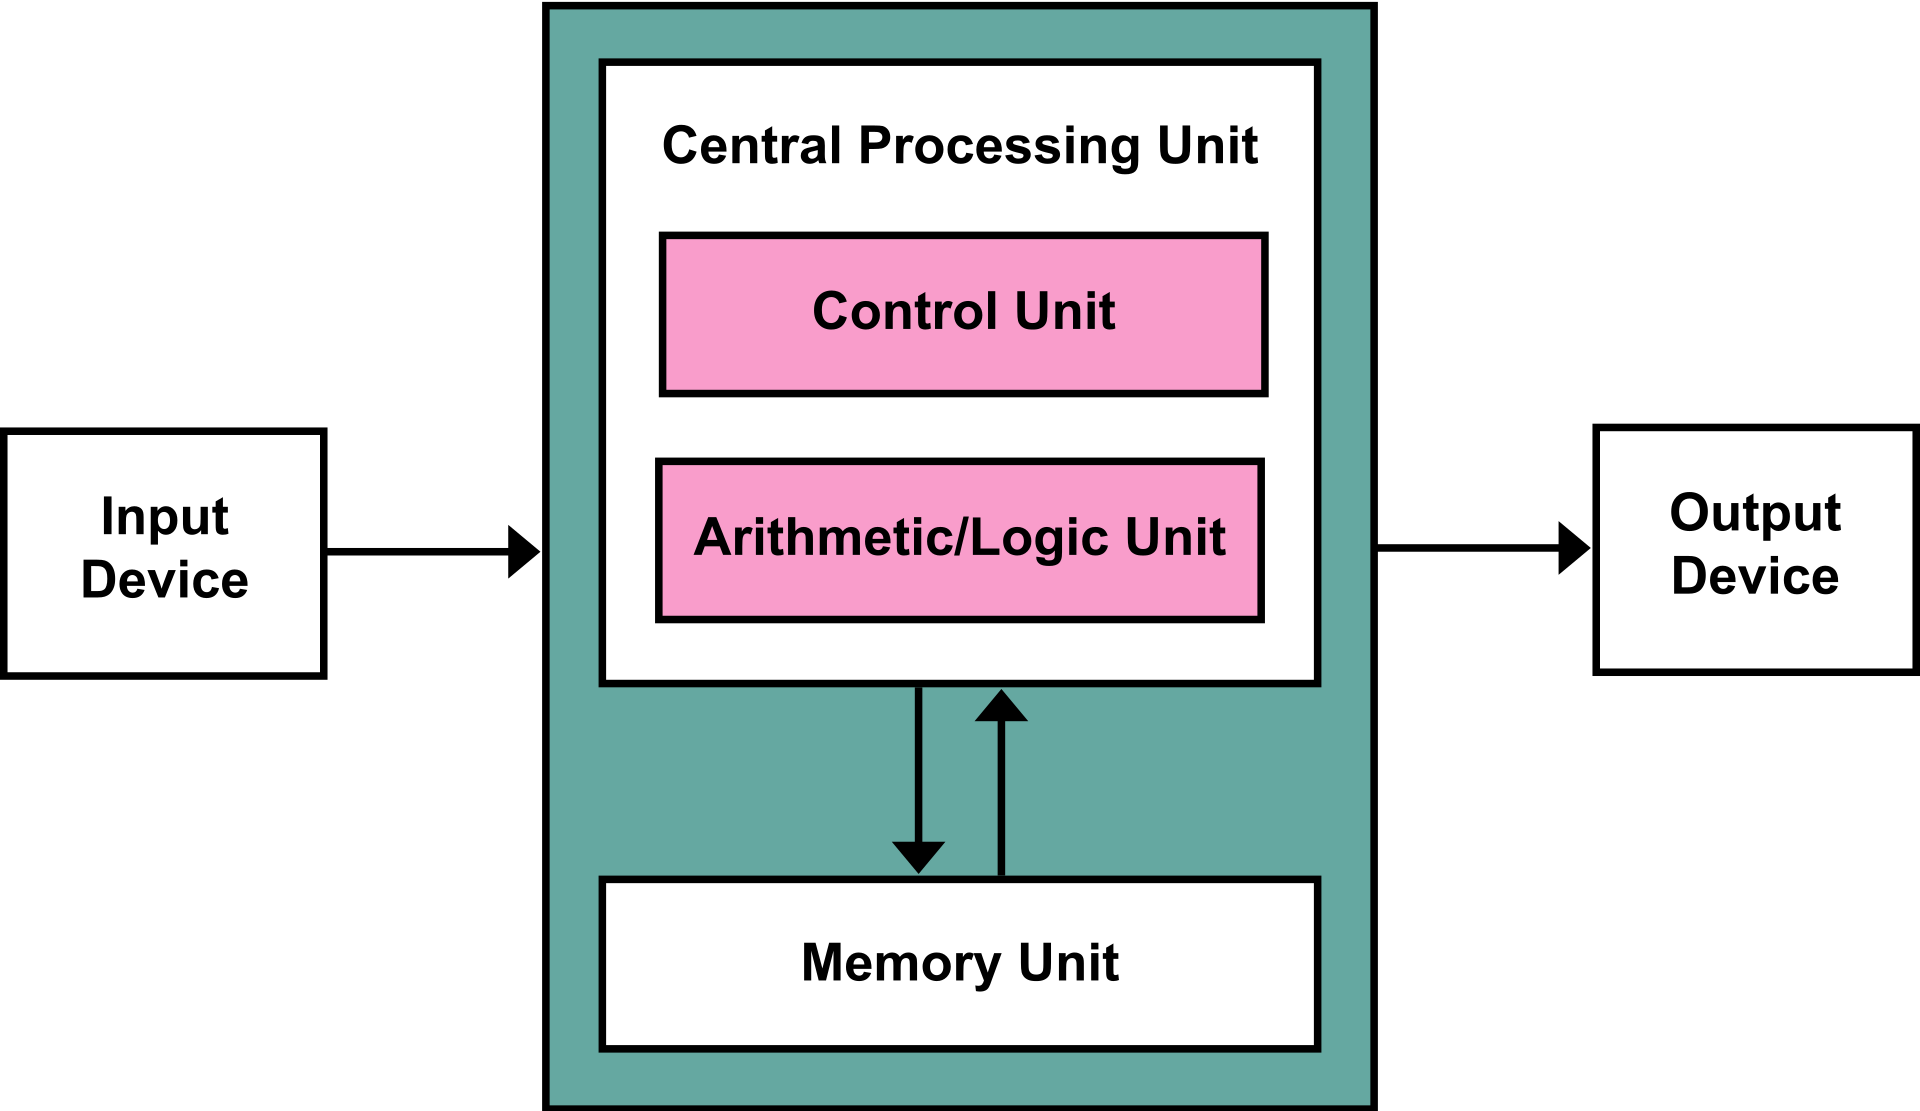
\includegraphics[width=0.95\textwidth]{./imgs/von-neumann-arch.png}
    \vfill
  \end{minipage}
  \pause
  \vfill
  \textbf{Lets got over what a path is.}
\end{frame}

\begin{frame}[fragile]
  \frametitle{The OS Module: Path}
  \begin{itemize}
    \item \lstinline|os.stat()| \textrightarrow \ Returns all information on a file.
    \item \lstinline|os.remove()| \textrightarrow \ Removes a file at a given path.
    \item \lstinline|os.path.isfile()| \textrightarrow \ Test whether a path is a regular file
    \item \lstinline|os.path.getsize()| \textrightarrow \ Return the size of a file, reported by os.stat().
  \end{itemize}
\end{frame}

\section{The OS Module}
\begin{frame}[fragile]
  \frametitle{The OS Module: Paths}
  \begin{itemize}
    \item \lstinline|os.path.split()| \textrightarrow \ Split a pathname.  Returns tuple "(head, tail)" where "tail" is everything after the final slash.  Either part may be empty.
    \item \lstinline|os.path.exists()| \textrightarrow \ Test whether a path exists.  
    \item \lstinline|os.path.isfile()| \textrightarrow \ Test whether a path is a regular file
    \item \lstinline|os.path.getsize()| \textrightarrow \ Return the size of a file, reported by os.stat().
    \item \lstinline|os.path.sep| \textrightarrow \ Gives you the separator characer that is used on your system.
  \end{itemize}
  \vfill
  \pause
  \textbf{Why do we need these?}
\end{frame}

\begin{frame}[fragile]
  \frametitle{Poll Question: Opening a File}
  How many times will this function call iterate if placed in a for loop: \lstinline|os.walk("dev_website")|?
  \begin{lstlisting}
  dev_website
  |---index.html
  |___elements
      |--- about.html
      |--- cv.html
      |___ projects.html
  \end{lstlisting} 
  \vfill
  \begin{enumerate}[A]
    \item 1
    \item 2
    \item 6
    \item 0
  \end{enumerate}
\end{frame}

%
% Slide 2
%
\section{Reading Files}
\begin{frame}[fragile]
  \frametitle{Poll Question: Opening a File}
  By default what does the \lstinline|open()| function have it's file access permissions set as?
  \begin{lstlisting}[language=Python, autogobble]
  \end{lstlisting}
  \vfill
  \begin{enumerate}[A]
    \item \lstinline|Reading|
    \item \lstinline|Writing|
    \item \lstinline|Appending|
    \item \lstinline|Reading and Writing|
    \item \lstinline|Writing and Appending|
    \item \lstinline|Reading, Writing, and Appending|
  \end{enumerate}
\end{frame}

%
% Slide 2
%
\begin{frame}[fragile]
  \frametitle{Files}
  Which of the following reads all the contents of a file into a list of strings?
  \vfill
  \begin{enumerate}[A]
    \item readlines
    \item readall
    \item read
    \item readline
  \end{enumerate}
\end{frame}


%
% Slide 2
%
\begin{frame}[fragile]
  \frametitle{Poll Question: Read Characters}
  Given a variable named \lstinline|file_object| that contains a file object which of the following will read the next 15 character into a variable named \lstinline|title|.
  \vfill
  \begin{enumerate}[A]
    \item \lstinline| title = file_object.read(15)|
    \item \lstinline| title = file_object.read(14)|
    \item \lstinline| title = file_object.reads(15)|
    \item \lstinline| title = read(file_object, 15)|
  \end{enumerate}
\end{frame}

%
% Slide 2
%
\begin{frame}[fragile]
  \frametitle{Reading from Files}
  \begin{lstlisting}[language=Python, autogobble]
  file_object = open('filename')
  lines = file_object.readlines()
  for line in lines:
    print(line)
  file_object.close()
  \end{lstlisting}
\end{frame}

\section{Write Files}
%
% Slide 2
%
\begin{frame}[fragile]
  \frametitle{Poll Question: Files}
  Continue writing to existing files without overwriting the contents of the original file?
  \vfill
  \begin{enumerate}[A]
    \item \lstinline|outf = open('filename', 'r')|
    \item \lstinline|outf = open('filename', 'x')|
    \item \lstinline|outf = open('filename', 'a')|
    \item \lstinline|outf = open('filename', 'w')|
    \item \lstinline|outf = open('filename', 'w+')|
  \end{enumerate}
\end{frame}

%
% Slide 2
%
\begin{frame}[fragile]
  \frametitle{Poll Question: Files}
  Read from a file that may not exist?
  \vfill
  \begin{enumerate}[A]
    \item \lstinline|outf = open('filename', 'r+w')|
    \item \lstinline|outf = open('filename', 'rw')|
    \item \lstinline|outf = open('filename', 'r')|
    \item \lstinline|outf = open('filename', 'r+')|
    \item \lstinline|outf = open('filename', 'w+')|
  \end{enumerate}
\end{frame}



%
% Slide 2
%
\begin{frame}[fragile]
  \frametitle{Writing to Files}
  \begin{lstlisting}[language=Python, autogobble]
  file_object = open('filename', 'w')
  file_object.write('thing to write')
  file_objet.close()  #automatic at program end
  file_object.flush() #optional
  \end{lstlisting}
\end{frame}

%
% Slide 2
%
\section{Patterns Continued}
\begin{frame}[fragile]
  \frametitle{Finding (single thing) in a Collection}
  \begin{lstlisting}[language=Python, autogobble][language=Python, autogobble]
  def find_thing(collection):
    for thing in collection:
      if <thing meets condition>:
        return thing
  \end{lstlisting}
  \vfill
  \begin{lstlisting}[language=Python, autogobble][language=Python, autogobble]
  def find_thing(collection):
    found = None
    for thing in collection:
      if <thing meets condition>:
        found = thing
        break
    return found
  \end{lstlisting}
\end{frame}

%
% Slide 2
%
\begin{frame}[fragile]
  \frametitle{Filtering a collection}
  \begin{lstlisting}[language=Python, autogobble][language=Python, autogobble]
  def filter(collection):
    new_list = []

    for thing in collection:
      if <thing meets criteria>:
        newlist.append(thing)

    return new_list
  \end{lstlisting}
\end{frame}

%
% Slide 2
%
\begin{frame}[fragile]
  \frametitle{Patterns and Files}
  \begin{minipage}{0.38\textwidth}
    Usual Sum/Total:
    \begin{lstlisting}[language=Python, autogobble]
    def foo(some_list):
      total = 0
      for item in some_list
        total += item
      return total
    \end{lstlisting}
  \end{minipage}
  \hfill
  \begin{minipage}{0.58\textwidth}
    Sum/Total Pattern w/ File:
    \begin{lstlisting}[language=Python, autogobble]
    def foo(filename):
      file_object = open(filename)
      lines = file_object.readlines()
      total = 0
      for line in lines:
        total += int(line)
      return total
    \end{lstlisting}
  \end{minipage}
\end{frame}


\end{document}
